\documentclass{article}

\usepackage[margin=1in]{geometry}
\usepackage{mathtools} %also loads amsmath
\usepackage{amssymb, bbm}
\usepackage[backend=biber,
	style=alphabetic,
	%	citestyle=authoryear,
	natbib=true,
	url=true, 
	doi=true]{biblatex}

%\usepackage{blkarray} % for matrices with labels
\usepackage{microtype}
\usepackage{relsize}
\usepackage{environ}% http://ctan.org/pkg/environ; for capturing body as a parameter for idxmats
\usepackage{tikz}
	\usetikzlibrary{positioning,fit,calc, decorations, arrows, shapes, shapes.geometric}
	\pgfdeclaredecoration{arrows}{draw}{
		\state{draw}[width=\pgfdecoratedinputsegmentlength]{%
			\path [every arrow subpath/.try] \pgfextra{%
				\pgfpathmoveto{\pgfpointdecoratedinputsegmentfirst}%
				\pgfpathlineto{\pgfpointdecoratedinputsegmentlast}%
			};
	}}
	%%%%%%%%%%%%
	
	\tikzset{dpadded/.style={rounded corners=2, inner sep=0.9em, draw, outer sep=0.4em, fill=gray, fill opacity=0.08, text opacity=1}}
	\tikzset{active/.style={fill=blue, fill opacity=0.1}}
	\tikzset{square/.style={regular polygon,regular polygon sides=4, rounded corners = 0}}
	\tikzset{octagon/.style={regular polygon,regular polygon sides=8, rounded corners = 0}}
	
	
	\tikzset{alternative/.style args={#1|#2|#3}{name=#1, circle, fill, inner sep=1pt,label={[name={lab-#1},gray!30!black]#3:\scriptsize #2}} }
	
	
	\tikzset{bpt/.style args={#1|#2}{alternative={#1|#2|above}} }
	\tikzset{tpt/.style args={#1|#2}{alternative={#1|#2|below}} }
	\tikzset{pt/.style args={#1}{alternative={#1|#1|above}} }
	

	\tikzset{mpt/.style args={#1|#2}{name=#1, circle, fill, inner sep=1pt,label={[name={lab-#1},gray]\scriptsize #2}} }
	\tikzset{pt/.style args={#1}{name=#1, circle, fill, inner sep=1pt,label={[name={lab-#1},gray]\scriptsize #1}} }
	
		
		 %\foreach \x in {#1}{(\x) (lab-\x) } 
		 
	\tikzset{Dom/.style args={#1 (#2) around #3}{dpadded, name=#2, label={[name={lab-#2}] #1}, fit={ #3 } }}
	\tikzset{Dom/.style args={#1 (#2) around #3}{dpadded, name=#2, label={[name={lab-#2}] #1}, fit={ #3 } }}
	\tikzset{bDom/.style args={#1 (#2) around #3}{dpadded, name=#2, label={[name={lab-#2}]below:#1}, fit={ #3 } }}
	\tikzset{arr/.style={draw, ->, thick, shorten <=3pt, shorten >=3pt}}
	\tikzset{archain/.style args={#1}{arr, every arrow subpath/.style={draw,arr, #1}, decoration=arrows, decorate}}
	%\tikzset{every label/.append style={text=red, font=\scriptsize}}
	
%	\newcommand\tikzdom[#1;#2](#3,#4[#5]){
%		\foreach [evaluate=\x as \y using (\x-#2/2)/#5 + #3] \x in {0, 1, ..., #2} {
%			\node[bpt={#1\x | $\n_\x$}] at (\y,#4) {};
%		}
%		\node[Dom={$\sf W$ (W) around \lab{w1}\lab{w3}}] {};
%	}

\usepackage{color}
\definecolor{deepgreen}{rgb}{0,0.5,0}

\usepackage[colorlinks=true, citecolor=deepgreen]{hyperref}


\setlength{\skip\footins}{1cm}
\setlength{\footnotesep}{0.4cm}

\usepackage{parskip}
\usepackage{amsthm, thmtools}
\usepackage{
	nameref,%\nameref
	hyperref,%\autoref
	% n.b. \Autoref is defined by thmtools
	cleveref,% \cref
	% n.b. cleveref after! hyperref
}

\begingroup
\makeatletter
\@for\theoremstyle:=definition,remark,plain\do{%
	\expandafter\g@addto@macro\csname th@\theoremstyle\endcsname{%
		\addtolength\thm@preskip\parskip
	}%
}
\endgroup
\makeatother

\theoremstyle{plain}
\newtheorem{theorem}{Theorem}[section]
\newtheorem{coro}{Corollary}[theorem]
\newtheorem{prop}[theorem]{Proposition}
\newtheorem{lemma}[theorem]{Lemma}
\newtheorem{fact}[theorem]{Fact}
\newtheorem{conj}[theorem]{Conjecture}

\theoremstyle{definition}
\newtheorem{defn}{Definition}[section]
\newtheorem{examplex}{Example}[section]
\newenvironment{example}
	{\pushQED{\qed}\renewcommand{\qedsymbol}{$\triangle$}\examplex}
	{\popQED\endexamplex\vspace{-1em}\rule{1cm}{0.7pt}\vspace{0.5em}}

\theoremstyle{remark}
\newtheorem*{remark}{Remark}

\usepackage{xstring}
\usepackage{enumitem}

%\newcommand\duplicat[1]{\gdef\mylist{}\foreach \x in {#1}{\xdef\mylist{\mylist (\x) (lab-\x) }}\mylist} %% this doesn't work :((
\newcommand\lab[1]{(#1)(lab-#1)}


\newcommand{\todo}[1]{{\color{red}\large\textbf{[todo}: {\normalsize\itshape#1}\textbf{]}}}
\newcommand\geqc{\succcurlyeq}
\newcommand\leqc{\preccurlyeq}
\newcommand\mat[1]{\mathbf #1}
\newcommand{\indi}[1]{\mathbbm{1}_{\left[\vphantom{\big[}#1 \vphantom{\big]}\right]}}
\newcommand\m[1]{\mathbf m_{\mathsf #1}}

\newcommand\recall[1]{ Recall \expandarg\cref{rex:#1}:\vspace{-1em} \begingroup\small\color{gray!80!black}\begin{quotation} \expandafter\csname rex:#1\endcsname* \end{quotation}\endgroup }

%OMG THIS WORKS

\def\wrapwith#1[#2;#3]{
	\expandafter#2{\expandarg\StrBefore{#1}{,}}
	\expandarg\StrBehind{#1}{,}[\tmp] 
	\xdef\tmp{\expandafter\unexpanded\expandafter{\tmp}}
	#3
	\expandarg\IfSubStr{\tmp}{,}{\wrapwith{\tmp}[#2;{#3}]}{ \expandafter#2{\tmp} }
}
\def\hwrapcells#1[#2]{\wrapwith#1[#2;&]}
\def\vwrapcells#1[#2]{\wrapwith#1[#2;\\]}



\newsavebox{\idxmatsavebox}
\def\makeinvisibleidxstyle#1#2{\phantom{\hbox{#1#2}}}
\newenvironment{idxmat}[3][\footnotesize\color{gray}\text]{%
	\def\idxstyle{#1}
	\def\colitems{#3}
	\def\rowitems{#2}
	\begin{lrbox}{\idxmatsavebox}$
	\begin{matrix}  \begin{matrix} \hwrapcells{\colitems}[\idxstyle]  \end{matrix} \\[0.1em]
		\left[ 
		\begin{matrix}
			\hwrapcells{\colitems}[\expandafter\makeinvisibleidxstyle\idxstyle]  \\[-1em]
	}{
		\end{matrix}\right]		&\hspace{-0.5em}\begin{matrix*}[l] \vwrapcells{\rowitems}[\idxstyle] \end{matrix*}
	\end{matrix}
	$\end{lrbox}
	\raisebox{0.75em}{\usebox\idxmatsavebox}
%	\vspace{-0.5em}
}

\newenvironment{sqidxmat}[2][\footnotesize\color{gray}\text]
	{\begingroup\idxmat[#1]{#2}{#2}}
	{\endidxmat\endgroup}

\usepackage{ wasysym }

\addbibresource{../refs.bib}
\addbibresource{../maths.bib}


\newcommand{\mfem}{\mathclap\female\male}
\newsavebox{\hourglassbox}
\savebox{\hourglassbox}{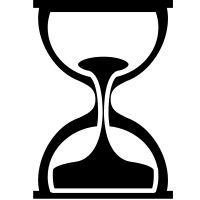
\includegraphics[height=.8em]{hourglass.png}}
\newcommand\hourglass{\usebox{\hourglassbox}}

\newcommand\modelname{{\color{blue!50!black}$\langle$\itshape model name$\rangle$ }}

\title{Discussion of \todo{need name for model} Semantics and Consistency}
\author{Oliver Richardson  \texttt{oli@cs.cornell.edu}}


\begin{document}
	\maketitle

%	\section{The problem with expressing impact as conditional probability.}
%	
%	When we say we have a domain of ``goodness'' $\sf U$, and a conditional probability distribution $\Pr(U \mid A)$, we are not expressing the goodness of $A$, rather estimating the goodness of the world where $A$ takes on various values. This is obviously a belief, and does not work as an expected utility calculation.  How to fix?
%	
%	\subsection{Add more nodes: a separate node for each component}
%	\subsection{Change impact arrows to be functions.}


%	Suppose that we have a diagram
%	
%	\begin{tikzpicture}
%		\node[dpadded](X){$X$};
%		\node[dpadded](A) at (-1, -1.3) {$A$};
%		\node[dpadded](B) at (1, -1.3) {$B$};
%		\node[dpadded](U) at (0, -2.6) {$U$};
%	\end{tikzpicture}

%	Goal: learn preferences over variables, which changes as slowly as possible, to be used in prediction. The classical picture of decision theory is a limit point with infinite cognitive power. You have to coordinate the different levels of preferences, and be very careful to avoid conflicts. 

%	\section{A Defense of  Semantics.}
	Recall that we have a model of nodes, chained together with Markov kernels / conditional probability distributions / stochastic matrices. Of course, there is already an enormous literature about diagrams which look somewhat like this, made up of nodes and conditional probability tables: Baysian Networks (BNs) and their many variants. The diagrams that we employ look very similar, but are intended for a different purpose, and hence have a different semantics. Whereas BN's are a factorization of a particular joint probability distribution and consistent by design, these models are merely constraints on the distribution, which might be so strong so as not to admit any joint distribution.
	
	We will go into the difference more carefully in the next section, but first here are some reasons to prefer this as a way of modeling agents,% in the order of explanation rather than importance:
	
	\begin{enumerate}[nosep]
		\item This representation more naturally matches what humans are aware of, encoding small locally consistent models rather than one giant probability distribution (see sections \ref{sec:human-belief-marginals},\ref{sec:human-pref-marginals})
		\item It is cleaner from a mathematical standpoint: utilities and probabilities are related, we get a notion of belief composition, and we can make use of both category and information theory (sections \ref{sec:util-prob-relate}, \ref{sec:composition}, and \ref{sec:belief-typing}).
		\item This allows composition of arrows to be defined, and gives meanings to paths (section \ref{sec:composition}).
		\item When bits of these diagrams are added and removed, the meaning and form of the rest of the diagram remains the same (section \ref{sec:diagram-alterations}).
		\item We can now represent inconsistency, which we will use to drive preference change. While we agree with the classical picture in that inconsistency is bad, now we can talk about it
		\item Due to the compositionality, it is possible to add typing rules to dynamically change beliefs, knowledge representations, and so forth (section \ref{sec:belief-typing})
		\item It is a strictly more general representation--- we can easily convert BNs to these diagrams (section \ref{sec:convert2bn})
	\end{enumerate}

	\subsection*{Recap: \modelname Definitions and Semantics}
	\begin{defn}
		A \modelname model $(\cal A, L)$ is a collection of variables $\cal A$, attached to each of which is some preference information: (this could be an order, utility, pairwise utility matrix, a supremum function), plus a collection of probabilistic links $\cal L$ between some (but not necessarily all) pairs of them, where $L: A\to B \in \cal L$ is a (sub) Markov kernel $A \to \Delta (B \cup \{\bullet\})$\footnote{The additional ``phantom element'' $\bullet$ absorbs probability density that we don't want to equivocate on, allowing our model to capture partial families of conditional probabilities, by extension things like implication, and giving agents more tools to avoid inconsistency. This has the effect of making our links substochatic matrices/kernels rather than stochastic ones. However, if we restrict to beliefs which assign zero probability to $\bullet$, everything in the model works as before. See section \ref{sec:substochastic} for details} representing beliefs about how a setting of $A$ to $a \neq \bullet$ will impact the value of $B$. 
	\end{defn}

	Variables can be thought of equivalently as:
	\begin{itemize}[nosep]
		\item random variables $X$ which can take on values $\{x_i\}$ (or possibly none, which we denote $\bullet$)
		\item sets $X$ with elements $\{x_i\}$
		\item partitions of the universe of outcomes into disjoint (but possibly not exhaustive) events $\{x_i\}$
	\end{itemize}
	
	In this document, we will focus on models where the preference information is encoded as a special utility domain $U$, with links from other variables. While there may be some propositions tying this case to utilities or preference orders, we will avoid talking explicitly about the more general setting of preference matrices and choice functions out for now.
	
	
	\section{Defense of \modelname as a Static Representation }
	\subsection{The Possibility of Type Constructors / Embedded Logic}\label{sec:belief-typing}
	The classical picture also features a fixed set of variables. In addition to allowing new concepts to form for exogenous reasons, we would like to have inductive ways of introducing new ones logically, as combinations of the existing variables. Interpreting variables as types, whose possible assignments are terms, the syntax of which variables we can construct and what beliefs we have about the resulting picture is a type theory. There are some obvious ways one might want to combine existing domains; the one we are concerned with here is products.
	
	In terms of beliefs, you might already have beliefs about how likely two  $A$ and $B$, then suddenly wonder about how they interact. For instance, you may already have beliefs about how likely you are to leave your keys in the ignition, and also how often your car is dead, and then wonder if there's a connection. 
	In terms of preferences, you might think $a \geqc a'$ and $b \geqc b'$, but now wonder what you would do if you had to choose between $a b'$ and $a' b$. In both cases, you are slightly enlarging your picture to consider the relevant features that a classical agent would already have.
	
	For this reason, we introduce the ability to create a domain $A \times B$, if $A$ and $B$ are nodes in the picture, whose elements are the cartesian product of $A$ and $B$. %Moreover, this comes with projection links $\pi_A : A \times B \to \Delta(A)$, $\pi_B: A\times B \to \Delta B$ given by $\pi_A((a,b), a') = \delta_{a,a'}$ and $\pi_B((a,b), b') = \delta_{b,b'}$, as usual. Furthermore, we can construct a function $\langle f , g \rangle : X \to A \times B$ for any $f: X \to A$ and $g: X \to B$ that make the picture no more inconsistent.
	This is represented graphically as:
	\begin{center}
		\begin{tikzcd}
%			&X\ar[dl,"f"']\ar[dr,"g"]\ar[d, "{\langle f, g \rangle}"description ]  \\
			A & A \times B \ar[l, "\pi_A"]\ar[r, "\pi_B"'] & B
		\end{tikzcd}
	\end{center}
	
%	It may be worth noting that we can always construct $\langle f, g \rangle$, but uniqueness in general does not hold, so it is not (yet) a categorical product.
	
	\subsubsection{Products vs Unions}
	
	We could have achieved a similar thing by considering $\{A\}$ and $\{B\}$ as singleton sets of variables, and then adding $\{A,B\}$ to the picture. Here we would interpret as a set of random variable taking values in the range of the product of its elements possible values. The two accounts differ when there is an overlap between the sets. Should we be allowed to represent $A \times A$? 
	
	Taking unions does protect us from doing certain bad things: it would be a mistake to assign a distribution $\Pr(a, a') > 0$ for $ a \neq a'$, for instance --- but we're already in the business of allowing this kind of inconsistency --- in the picture below all the marginals are fine as far as the syntax is concerned, but there is no way to assign a probability distribution on all of the nodes.
	\begin{center}
		\begin{tikzcd}[dpad]
			&1 \ar[d, "p(A\times A)"] \\
			 & A \times A \ar[ld]\ar[rd] & \\
			 A \ar[rr,equal]&& A
		\end{tikzcd}
	\end{center}

	It can also be very useful to keep extra copies of $A$ around even if (part of) one already exists buried in another variable, because we can delay integration using this trick, as in example \ref{ex:bayesrule} for instance. The most compelling reason for me is that one might not know that you're looking at two copies of $A$; maybe they've been framed differently --- but still you should be able to take a product and get two things, rather than a union, which immediately leaks the truth of their equivalence to an agent.
	
	\subsubsection{Additional Types}
	\todo{Gestures towards embedding logics; equivalence between logic and type theory; in particular: conditionals, coproducts, negation, higher order nodes (beliefs about prefs, prefs about beliefs)}	
	
	% Motivating example: why do we need A x B?  Why not just have a BN?
	%	If $A$ and $B$ are random variables, 
	
	
	
	
	
	\subsection{Converting BNs}\label{sec:convert2bn}
	The semantics of a Baysian network ensure that there is no inconsistency: the arrows into a node taken together collectively determine a single well-defined probability distribution. Formally they consist of a set of nodes $\cal N$, and for each $N \in \cal N$, a set of parents $\mathrm{Par}(N)$, and a conditional probability distribution $\Pr( N \mid \mathrm{Par}(N))$, which is a distribution over the values of $N$ for each setting of every variable in $\mathrm{Par}(N)$. While each of our arrows can be interpreted by itself as a marginal, a collection of arrows into a single node must be taken together to have any meaning in a BN. 
	
	The procedure for converting to a BN is simple: we simply take every node's incoming arrows, and insert the product of its parents as a node before it. With this procedure, if a node $N$ has just one parent $P$, we replace $P \to N$ with $P \to N ~=~ N$, which is redundant so we don't draw this. If a node had zero parents (i.e., the BN just gives it a probability distribution not dependent on anything), we insert the product of zero things, i.e., the singleton node $1 = \{*\}$, a variable which only takes one value, and set $\Pr(N \mid *) = \Pr(N)$. 
	
	This sound much more complicated than it is. Consider the example below, where the left is a BN, and the right is the corresponding \modelname.
	\begin{center}
		
		\begin{tikzcd}[center base, column sep=2.5em]
			& A \ar[dl]\ar[dr] \\
			B \ar[dr] && C \ar[dl]\\
			& D &
		\end{tikzcd}
		\hfil
		\begin{tikzcd}[center base, column sep=2em, dpad]
			& \mathsf 1 \ar[d] &\\
			& A \ar[dl]\ar[dr ]% \ar[dd,dashed, gray] 
			\\
			B && C \\
			& B \times C \ar[ul, gray!70] \ar[ur, gray!70]\ar[d] & \\
			& D &
		\end{tikzcd}
	\end{center}
	\vspace{0.5em}

	We have effectively changed two things: first, visually encoded the probability distribution of $A$ as the arrow $1 \to A$ (which we are now allowed to omit; sometimes you don't want priors on things, such as your own actions). Second, we have combined the two arrows $B \to D$ and $C \to D$ into a single one, $B \times C \to D$. Though certainly more verbose, this is arguably visually clearer if want to follow arrows: you cannot compute $D$ from $B$; you need both $B$ and $C$.
	
	In order to fully get the joint representation given by the BN we would also need to make the final assumption that $B \CI C \mid A$. This is possible to do with an extra arrow, but this solution doe not scale well and clutters the diagram. Instead, we will leave the picture as it is, and tackle the independence in a weaker way.
	
	\begin{defn*}
		The \emph{center} of a \modelname $(\cal A, L)$ is the set of joint distributions on $\cal A$ that come closest to satisfying $\cal L$, which are of maximum entropy.
	\end{defn*}

	This is an alternate way of capturing the conditional independence of variables that are not required by the model to be related, without ever conditioning on ancestors, which include products\footnote{to see why this is problematic, consider that the product of all variables can always be formed, and is the ancestor of all variables. If we condition on it, then everything is always conditionally independent, as we're looking at a degenerate distribution consisting of a single outcome.}.  In some sense this is the worst case outcome for an agent intending to narrow down possibilities: a distribution in the center requires the maximum amount of information to determine the state of the world, but at the same time cannot leverage this assumption to simplify things. The principle of maximum entropy is well established\footnote{Despite this, utilities are still thought of as fixed, minimum entropy objects.} \todo{choose references}. We also get:
	
	
	\begin{restatable}{theorem}{rthm:bn-maxent} \label{rthm:bn-maxent}
		The center of the \modelname obtained by transforming a Bayesian Network as described above (i.e., by inserting an extra node $X := \prod_{P \in \mathrm{pa(A)}} P$ before every node, with the appropriate projections), is a singleton set consisting of exactly the probability distribution that the BN represents.
	\end{restatable}

	\begin{coro}
		Products (defined in section \ref{sec:belief-typing}) in the center of a model $(\cal A, L)$ have the usual uniqueness to make them categorical limits.
	\end{coro}

	We will clarify this definition and explain the connection to thermodynamics more carefully (section \ref{sec:thermo}) once we have a numerical definition of consistency. In the mean time, we continue to argue for this collection of marginals as a way of representing beliefs.

	
	% The BN makes the assumption that the value of $D$ cannot depend on anything else; we're only 
%	This also illustrates another important point: the assumptions that you make to drawn a BN, even if locally sensible, build on one another and might not end up being what you wanted to model. On the left it visually looks like you can estimate $D$ from
	% $B$, which is false. It also looks like you can estimate $D$ from 
%	$A$ --- which is true, but only if we've actually modeled all of the confounding factors! For instance, if $B$ has some small mostly negligible dependence on $C$ that we've failed to model, the estimation of $D$ can be arbitrarily bad, if it is sensitive to the correlation between $B$ and $C$.
	
	\subsection{Human Beliefs as Marginals}\label{sec:human-belief-marginals}
	From a modeling perspective, the biggest reason for keeping track of marginals rather than joint probability distributions, is that it can represent lots of information tracked by people, that BNs regard as incomplete. As seen earlier, the major feature we admit that is prohibited in a Baysian Network is a merging of two paths, where neither is a projection.
	
	In our case, we also have the possibility of branching and merging. In our picture, a diagram $A \rightarrow C \leftarrow B$ represents two probability distributions $\Pr(C\mid A)$ and $\Pr(C \mid B)$.
	Having this kind of information is both common and not representable as a (single) probability distribution. Scientific studies never control for everything that is relevant, so you're left with marginals which may not tell the whole story.
	
	\begin{example}
		After reading a number of empirical studies, you come to believe that smokers have a 70\% chance of developing cancer, compared to 20\% for non-smokers. At the same time, you believe that those who use tanning beds have a 80\% chance of developing cancer, compared to 18 \% for those who do not use them. You have no information about how the two interact.
	\end{example}
	
	\begin{example}
		You are on a game show, and offered a choice between several levers $(A)$; your choice will determine how much money you receive. You are uncertain what each lever does, but you do have a vague intuition about the mechanism, giving you a distribution over amounts for each lever ($\Pr(C \mid A)$). You also had enough time to read statistics about how well people have done in the past $(\Pr(C))$. You do not have any information about what levers they've chosen though, nor do you have a complete joint probability $\Pr(A, C)$. In fact, having an accurate probability on $A$ alone would seem to undermine your agency.
	\end{example}


	So information of this form may not be entirely complete, be contradictory, or make it seem as though the choice is an illusion. This ``outside view'' is also important for constructing Newcomb's problem:
	
	\begin{example}[Newcomb]
		There are two boxes. Box 1 is clear and visibly contains \$1k; box 2 is opaque, and will contain \$1M if a predictor (which you know has been very accurate in the past) predicts you will leave box 1, taking just this box, and will contain nothing if the predictor predicts you will take the first box. You have to choose whether or not to take the visible box (there's no reason not to take box 2).
		
		In the diagram below, you and your past choices determine the prediction $P$, as given by the blue line, but you do not have access to this information. They also determine your action $A$ in some sense, which is the right dashed arrow, which you only know for certain after you make your decision. Because the two processes cannot exchange information (i.e., the predictor cannot decide after your action has been made, and you don't get to know the prediction), these two processes determine the process $\mathrm{Identity} \to A \times P$.
		\begin{center}
			\begin{tikzcd}[dpad]
				& \text{Identity}\ar[dr, blue, dashed]\ar[dl, dashed]\ar[d,dotted, gray]\\
				\text{Action} & A \times P \ar[r]\ar[l]\ar[dl]\ar[d] & \text{Prediction} \\ \$\$ & A\stackrel{?}{=}P & \mathsf 1 \ar[l]
			\end{tikzcd}
		\end{center}
		Now, on the one hand, you have a logical picture of how an action and prediction together will impact whether the predictor is right (the arrow $A \times P \to A \stackrel{?}{=} P$). On the other hand, you also have an outside view of how likely the predictor is to be right (the arrow $1 \to A \stackrel{?}{=} P$). We have not resolved the paradox; we have merely represented the beliefs in the setup, which make very little sense as a BN.
%		More weirdness comes from the fact that $A$ and $P$ interact.
	\end{example}

	At least classically, beliefs are only half of the picture. Keeping around marginals is also more psychologically plausible for preferences.

	\subsection{Human Preferences as Marginals}	\label{sec:human-pref-marginals}
	In this section we will argue that the distinction between `pure' utilities and `expected' ones does not make much psychological sense. Clearly from a mathematical perspective the two are different: the pure utilities can be used to make sure the whole picture is consistent in the classical setting, and are unchanged by beliefs. In our view these are both bad things for modeling people, and drawing this distinction also causes the math to be less unified in subtler ways. In any case
	
	\begin{example}
		Suppose you really like ice cream, and assign high utility to it. But now your family and government collaborate to make sure that whenever you eat ice cream you get an unpleasant electric shock, and feel awful for a day. It's bad enough that it's definitely not worth eating ice cream. But in this new life of yours, do you like it? The classical answer is yes. You will always like ice cream, it's just that you dislike shock. But we know that experiences that co-occur blend into one another a lot; a bad meal or bad date can ruin a restaurant, and that's much more ephemeral than a shock collar that is now part of your life. It's even harder to argue this if you consider the collar being put on before you've ever had ice cream. Now ice cream tastes like pain, and you would avoid it either way.		
		
		It gets worse still: what if instead of an external device, the procedure was a hypnosis that made you feel this way? It seems hard to argue that the new version of you still likes ice cream.
	\end{example}

	When you can't separate two effects, there's no reason to talk about them, and no way to differentiate between them; such a representation should fade into the background. There's also no reason to restrict ourselves to trivial things such as tastes. The more important things, too (and perhaps especially, since they're further away from qualia) should be treated in context.
	
	\begin{example}
		You think freedom is objectively valuable. Governments and organizations that restrict freedom give worlds negative utility in your view, and tools that give people more freedom are of positive utility. But why do you like freedom? Presumably it's in part based on experience, and reading, and thinking about the structure of how societies are set up. It's not just a preference which comes from nowhere. If you lived in an alternate reality where people were much more malevolent and freedom was always associated with murder--- where free societies collapsed immediately and tools that empowered people were invariably used for evil--- would you still think freedom is good?
	\end{example}

	What you really mean when you say, colloquially, that something has high utility, or that you like one thing more than another, is that you like it \emph{in context}. It's not that you would universally like it to be true over the alternative, as CP nets assume, or that you have some fixed platonic additive component of a utility function inside of you that gives you some number of points for freedom, as the classical view of economics would suggest. We're really talking about expected utility --- or more generally, the marginal distribution of ``good'' given different choices, given your current beliefs. Even this insistence on collapsing the distribution to its mean is problematic, and makes problems like risk aversion trickier to talk about. The risk associated with not feeling good even though the state of the world is exactly what you thought it would be is almost never accounted for, and yet seems like a big deal, especially for people who don't have clear purpose in life.
	
	We can now get back to more technical benefits of looking at the world as a collection of conditional distributions.

	\subsection{Composition Of Arrows} \label{sec:composition}
	One feature we really would like to have is the ability to chain these conditional distributions together. Among other things, a well-behaved notion of composition will:
	\begin{itemize}[nosep]
		\item give meanings to the visual paths
		\item allow us to represent integrating out variables graphically
		\item unlock parallels to other structures through category theory
		\item think of expected utility, belief propagation, and inductive inference as simple juxtapositions of arrows
	\end{itemize} 
	
	Since arrows are Markov kernels / matrices, we already have a natural way of doing this, by integration / summation over the intermediate variable --- if $f : A \times B \to \mathbb R$ and $g : B \times C \to \mathbb R$ (this is the finite case) we can obtain a stochastic matrix
	
	\[ g\circ f : A \times C \to \mathbb R =  \sum_{b \in B} f( b \mid a) g(c \mid b) \]
	
	So are we done? We now have a notion of composition that lines up with matrix multiplication and gives us a marginal of the appropriate kind. Unfortunately, there are a few good reasons people are deterred from this formulation. 
%	For Markov chains, the state of $B$ entirely determines the state of $C$, and so if $f = p(B \mid A)$ and $g = p(C \mid B)$, $g\circ f = p(C \mid A)$. 
	

	
	\subsubsection{Should paths be equal?}
	
	This design decision also has the effect of proving multiple ways to calculate things, which leads to the somewhat counter-intuitive fact that that not all diagrams commute, even ignoring preferences entirely. We will begin by explaining why this might not be what one would expect. 
	\begin{enumerate}
		\item Markov processes behave this way, and most things can be modeled as Markov processes. Unfortunately, to do this, we require control over the state representation --- and many of our variables might have way less information capacity than would be required to make this work.
		\item If your distribution can be described as a Bayesian network without any merging, then all diagrams commute (this is simply a result of the associativity of composition).
		\item If everything were deterministic, all diagrams would commute
		\item Even in our setting, many of them have to commute, and in fact several axioms of probability can be expressed as requirements that large classes of them must.
	\end{enumerate}

	
	\begin{example}[Marginalization] \label{ex:margin}
		Recall how a probability can be obtained by marginalization:
		\[ p(b) = {\color{gray}\sum_{a \in A} p(a \land b) = \sum_{a \in A} p(a) \frac{p(a\land b)}{p(a)} }= \sum_{a \in A} p(a) p(b\mid a) \]
		below is an illustration of this fact:
		\begin{center}
			\begin{tikzcd}[dpad]
				& 1 \ar[ld, "p(A)"']\ar[rd, "p(B)"] \\
				A \ar[rr]\ar[rr,"p(B \mid A)"'] &  & B\\
			\end{tikzcd}
		\end{center}
		The left part of the diagram represents the right side of the equation and vice versa. 
	\end{example} 

	This can be used inductively to show that every pair of paths from the singleton object $1$ is equivalent, but before that we will deal with another important case:
	
	\begin{example}[Bayes Rule] \label{ex:bayesrule}
		We can also represent Bayes' rule, $p(a \mid b) p(b) = p(b \mid a) p(a)$ as an assertion that two paths from:
		\begin{center}
			\begin{tikzcd}[dpad]
				&1 \ar[dl, "p(A)"']\ar[dr,"p(B)"]\\
				A \ar[dr, "p(B \times A \mid A)"'] & & B  \ar[dl, "p(B \times A \mid B)"]\\
				& B \times A 
			\end{tikzcd}
		\end{center}
		This can be seen as two applications of marginalization, one for each half. On the left, we have
		\[ p(b, a) = \sum_{a' \in A} p(a')p(a,b \mid a') = \sum_{a' \in A} p(a') p(b \mid a') \delta_{a,a'} = p(a) p(b \mid a) \]
		and similarly, the right gives $p(b,a) = p(b) p(a \mid b)$. One thing to take away is that one can avoid the integration over a variable by simply considering the conditional distribution to a different variable: namely, one which is the product of the input and output. 
	\end{example}
	
	
	However, not all paths generated by composition of probabilities are strictly equal! 
	
	\begin{example}
		In an extreme case, we can forget all of our information with the Markov assumption by going through a singleton object:
		
		\begin{center}
			\begin{tikzcd}[dpad]
				A \ar[rd]\ar[rr,"p(A\mid A) = \mathrm{id}_A"] &  & A\\&1 \ar[ru, "p(A)"']
			\end{tikzcd}
		\end{center}
	\end{example}
	
	For this to happen, the only thing we need is to allow composition and provide a probability on $A$; there's nothing inconsistent about this picture. Therefore, the measure of consistency is weaker than ``all paths are equal''. Still, there are some blatantly inconsistent pictures one could draw --- anything that violates Bayes' rule or marginalization, for example (see section \ref{sec:inconsistency-ex} for more).
	
	Our singleton example is a little bit annoying, but at least it's the best prediction that could be made after forgetting all of the information. It is natural to ask: is ignoring everything the \emph{worst} we can do? Is every bit of signal helpful? The answer is no. % There are two competing intuitions here: on the one hand, correlations are not transitive; on the other, if an intermediate variable $Y$ is positi
	
	\begin{example} \label{ex:badcommute}
		Men earn more than women, and people who earn more are generally older, but women live longer than men, so the top composition in the picture below
		\[ \begin{tikzcd}[dpad]
			& \$ \ar[rd] \\
			\mfem \ar[rr]\ar[ru] &&  \hourglass
		\end{tikzcd} \]
		is worse than ignoring all information and just predicting age. Here it is with numbers. Suppose the truth is a conditional probability distribution $\Pr(\$, \hourglass \mid\mfem)$ given by
		
		\begin{center}
		\begin{tabular}{r|ccccc|}
			\multicolumn{1}{c}{}&\multicolumn{2}{c}{\male}  &&\multicolumn{2}{c}{\female} \\
			&$<$40 yr & $\geq$40 yr &\vline& $<$40 yr & $\geq$40 yr \\\cline{2-6}
			$<\$40$k & .225 & .05 && .185 & .19 \\
			$\geq\$40$k & .075 & .15 && .065 & .06\\\cline{2-6}
		\end{tabular}
		\end{center}
		We can now construct our chain, $\mfem \to \$ \to \hourglass$
		\begin{center}
		\begin{tikzcd}[column sep=1.5cm,row sep=1.2cm]
			m \ar[r, ".55"]\ar[rd, ".45"description,pos=0.8] & <\$40k \ar[r,".63"]\ar[rd,".37"description,pos=0.8] & < \text{40 yr} \\
			f \ar[r, ".25"']\ar[ru, ".75"description,pos=0.8] & \geq \$40k \ar[r,".60"']\ar[ru, ".40"description,pos=0.8] & \geq \text{40 yr}
		\end{tikzcd}
		\end{center}
		Now, consider the following three arrows $\mfem \to \hourglass$, as estimates of $\Pr(\hourglass \mid \mfem)$:\\
		
		\begin{minipage}{.33\linewidth}\centering
			(1) the truth, $\Pr(\hourglass \mid \mfem)$:\\[1em]
			\begin{tabular}{c|cc}\hline
				& $<$40 yr & $\geq$40 yr \\\hline
				\male & .6 & .4 \\
				\female & .5 & .5 \\\hline
			\end{tabular}
		\end{minipage}
		\begin{minipage}{.33\linewidth}\centering
			(2) $\mfem\to 1\to \hourglass$:\\[1em]
			\begin{tabular}{c|cc}\hline
				& $<$40 yr & $\geq$40 yr \\\hline
				\male & .55 & .45 \\
				\female & .55 & .45 \\\hline
			\end{tabular}
		\end{minipage}
		\begin{minipage}{.33\linewidth}\centering
			(3) $\mfem\to \$\to \hourglass$:\\[1em]
			\begin{tabular}{c|cc}\hline
				& $<$40 yr & $\geq$40 yr \\\hline
				\male & .53 & .47 \\
				\female & .57 & .43 \\\hline
			\end{tabular}
		\end{minipage}
		\vspace{1em}
		
		We can see that $(2)$, which kills all signal, is closer to the truth than (3) in every way. Still, the picture is entirely consistent. Moreover, all of the important details of the joint distribution are saved in the three arrows, and subjectively, I used the arrows to construct the joint distribution I wanted, rather than the other way around.
		
		Even though this triangle does not commute, still every pair of paths from $1$ to another node are equivalent; for instance, marginalizing out gender gives the same distribution on age in all three of the cases above.
	\end{example}

	There are more persuasive examples using preferences. Multiple paths from a domain to $U$ can be thought of as pieces of a pros/cons list; in this case, people are intimately familiar with the fact that paths are not always equal.
	\begin{example}\label{ex:procon}
		In expectation, if I eat this bagel, I'm less likely to be hungry, and when I'm not hungry, I'm likely to be happier. On the other hand, suppose I'm allergic to gluten, and if I eat the bagel, I'm also likely to be irritated and uncomfortable, and when irritated and uncomfortable, I'm likely to be less happy. 
		\begin{center}
			\begin{tikzcd}[dpad, row sep = 0.5em]
				& \text{Hungry}\ar[dr] \\
				\text{Bagel} \ar[ur]\ar[dr] && \mathsf U \\
				& \text{Irritated} \ar[ur]
			\end{tikzcd}
		\end{center}
		The two paths are opposite polarity and hence the two paths cannot be equal.
	\end{example}

	The very fact that we write down both pros and cons implies paths aren't in general equal. So. Why even bother with composition then, if it doesn't give you the truth? People still write down arguments in support of and refuting positions, and often this is helpful. In example \ref{ex:procon} the intuition is still that somehow by weighting the reasons appropriately and finding the centroid we're likely to reach a good decision.

	% Why bother with composition? composition does the right thing under markov assumption, and we can always move the representation in such a way that we can get a markov assumption.

	Also, as mentioned in the beginning of the section, we can do some cool things with composition. The beliefs we model clearly should not necessarily be closed under composition, but being able to form them is still useful:
	\begin{itemize}[nosep]
		\item In the absence of additional information, the composition of two links is in some sense the best available estimate, and is compatible with any distribution in the center of the \modelname.
		\item If multiple, disjoint paths, this is good evidence that the final estimate is good --- like obtaining the same value from two different fermi estimates.
		\item In some cases, the composition is guaranteed to equal or approximate the true probability.
	\end{itemize}

	\subsubsection{Some Results} \label{sec:commute-results}
	Still, path equality is often expected; we would like to characterize when and why. Below are some necessary conditions for consistency, although more exploration is required.
	
	\begin{prop}\label{prop:prob-eq}
		If $\pi$ is a path of conditional probabilities $1 = A_0 \to A_1\to\cdots \to A_N = X$, then the composition $\pi^\circ$ of links in $\pi$ is equal to $\Pr(X)$.
	\end{prop}
	\begin{proof}
		This can be done by induction on the result from example \ref{ex:margin}, which is also the base case. The inductive step is as follows: if there is some joint probability $p$, and $\pi^{\circ k} := 1 \to \cdots \to A_k = p(A_k)$, then since we've assumed $p(A_{k+1} \mid A_k) = \pi_k$, we also have 
		\[ \pi^{\circ k+1} = \sum_{a \in A_k} p(A_k)(a) p(A_{k+1} \mid A_k(a)) = p(A_{k+1}) \] again by the example.
	\end{proof}

	Similarly, we have the dual result for deterministic functions:
	\begin{prop}\label{prop:det-eq}
		If a variable $Q$ is completely determined by both $A$ and $B$, i.e., $g : A\to Q$ and $h : B\to Q$ are deterministic, and $f : A \to \Delta B$ is $\Pr(B \mid A)$, then $h \circ f = g$. 
	\end{prop}
	\begin{proof}
		If there is a non-zero probability that $A = a$ while $B = b$, then it must be the case that $g(a) = h(b)$, since both $a$ and $b$ determine $Q$. So
		\begin{align*}
			h \circ f(a,q) = \sum_{b \in B} f(a,b) \delta_{h(b),q}	
					= \sum_{b \in B} f(a,b) \delta_{g(a), q} 
					= \delta_{g(a),q} \sum_{b \in B} f(a,b) 
					= \delta_{g(a),q} 
					= g(a, q)
		\end{align*}
	\end{proof}'

	We can also use information theory to obtain some bounds. Degenerate, deterministic marginals (zero entropy) must commute, and because the paths are guaranteed to be centered (see how even in example \ref{ex:badcommute} the means of the three compositions are the same) the possible deviation between paths is bounded by the entropy of the components. As a result, we will be able to show something in the spirit of the following (though it probably needs some revision):

	\begin{conj}
		A composition of arrows can only be as far off as its entropy permits: if we have marginals $A \xrightarrow{L} B \xrightarrow{P} C$, then
		\[ \forall a \in A.~ \Big|  P\circ L (a) - \Pr(C \mid a) \Big|  \leq H(L) + H(P) \]
		where $\Pr$ is any distribution consistent with $L$ and $P$.
	\end{conj}
%	\begin{proof}
%		\[  H(L) + H(P) \geq \frac{1}{2}  \Big| H(\Pr(C \mid A)) - H( P \circ L) \Big | \]
%	\end{proof}

	To summarize: we have a picture containing conditional distributions, particularly the ones which are most useful and actionable. Each conditional is a constraint on the world. We have a natural way of composing distributions, but sometimes the composition of two distributions will not be consistent with the rest of your beliefs.
		
	\subsection{Altering Diagrams} \label{sec:diagram-alterations}
	
	\subsection{Relations between Utilities and Probabilities} \label{sec:util-prob-relate}
	\todo{This is in the other documents. I can lift it if this becomes something more stable and we want it here}
	
	\subsection{Sub-stochastic Transitions and Conditionals} \label{sec:substochastic}
	
	Often, an otherwise very useful variable might not apply. The variable describing whether or not your answer is correct doesn't make sense if you weren't solving problems; the amount of money in your wallet doesn't make sense if you don't own one, and so forth. So now, when you're trying to predict the probability of certain amounts of money in your wallet, some of the probability mass needs to go into the ``actually this doesn't make sense'' bucket. 
	
	Usually, this is not really a problem, because we can always just add that bucket as a real option that a variable can take: a variable which might not make sense can always take a \texttt{null} value, and so now the set of possibilities is once again exhaustive. For us, this resolution poses a problem: our marginals now require us to estimate the distribution of many things given a null value--- suppose you are trying to represent the belief that you're happier when you get the right answer as a marginal link $L[\mathrm{RightAns}\to \smiley]$. We now need a distribution on happiness when you get the right answer, when you get the wrong answer, and also for when the question doesn't apply. But why doesn't it apply? Are you not solving problems because you're skiing? Because you've been injured? Maybe you are solving problems but there are multiple right answers? You can't just answer with a prior over happiness if you want to have consistent beliefs, because solving problems and happiness might be correlated. To be fair, this is something you certainly \emph{could} have, but it's annoying that we cannot provide a belief about ``does the right answer make you happy?'' without also answering the much more difficult question, ``are you happier when `the right answer' is an applicable concept to your life?''.
	
	In addition to being psychologically implausible, it dramatically reduces the number of things we can represent; take implication, for instance. If $A, B$ are binary variables (taking values $a, \bar a$ and $b, \bar b$ respectively), we can easily represent $A = B$, $A = \lnot B$ as stochastic matrices
	
	\[ p(B \mid A) = \begin{idxmatphant}{$a$,$\bar a$}{$b$, $\bar b$}{} 1 & 0 \\ 0 & 1 \end{idxmatphant}
		\qquad\text{and}\qquad p(B \mid A) = \begin{idxmatphant}{$a$,$\bar a$}{$b$, $\bar b$}{} 0 & 1 \\ 1 & 0 \end{idxmatphant}
		 \]
	
	but you cannot (via stochastic matrices) believe that $A \Rightarrow B$ without also believing a prior over $B$ given $\bar a$. Maybe the best strategy is a uniform prior (principle of maximum entropy, used in theorem proving in \cite{logicalinduction}), but this makes your beliefs inconsistent if it happens that $B$ is always false for other, unrelated reasons. 
	
	For this reason, we drop the requirement that our null element, $\bullet$, indexes a distribution in marginals. Below is an example of transition matrix $A \to B$ including the extra element. As mentioned, the last row is not something we are keeping track of.
	
	\[ \begin{idxmat}{$a_0$, $a_1$, $a_2$, $\bullet$}{$b_0$, $b_1$,  $\bullet$}
		.2 & .1 & 0.7 \\
		0 & 0 & 1 \\
		1 & 0 & 0\\\hline
		{\color{gray}.2} & {\color{gray}.6} & {\color{gray}0}
	\end{idxmat} \]
	
	Furthermore, because the final column is just whatever is necessary to make the rows sum to 1, we don't need to keep that either; as a result, it is sufficient to keep a smaller matrix without any $\bullet$-indices; the only price that we pay is that this matrix is \emph{sub}-stochastic rather than stochastic: its row entries sum to at most 1, rather than exactly 1. Composition works just as before; the product of sub-stochastic matrices is sub-stochastic.
	
	There is no way to get a Bayesian Network to do this, because we require the look-up tables to exactly match all possible values, so we get a real distribution at the end, rather than a weaker sub-distribution.
	
	There are several other technical results that we will eventually need to make sure that no tricks are being pulled when we later use standard formulae for probability distributions, but I'm going to skip fully typesetting and verifying them for now.
	
	\subsubsection{Substochastic Sanity Results} 
	\todo{show we can still use Bayes rule, marginalization etc., under certain circumstances. Most should follow just by adding $\bullet$ as an absorbing state and interpreting in a larger space}

	
	\section{Inconsistency}\label{sec:inconsistency-ex}
	% This is a predicate definition. We would also like to have a continuous definition so we can do gradient descent. 
	We will start with a simple predicate definition of \modelname consistency, of preference consistency, and give some examples before stating a less-brittle continuous generalization that will allow us to deal with inconsistent models.
	
	\begin{defn}[consistency]
		A \modelname $(\cal A, L)$ is \emph{consistent} if there exists some joint probability $\Pr(\cal A)$ on all of the variables, that is consistent with every link marginal $L \in \cal L$.
	\end{defn}


	\begin{defn}
		A \modelname $(\cal A, L)$, in which preferences are represented by a single utility node $U \in \cal A$, is \textit{pref-inconsistent} if it is inconsistent, but only because of the utility node --- i.e., the model obtained by deleting $U$ and all links to it, $\big(\mathcal A \setminus U,~~\mathcal L \setminus \{ L : \square\to U \}\big)$ is consistent.
	\end{defn}

	We will now show how they correspond to other intuitions of inconsistent preferences through some examples and specific cases.
	
	\subsection{Intransitivity of Preferences as Inconsistency}
	

	
	While restricting ourselves to use preferences represented by a utility domain, we cannot represent intransitive preferences directly in the usual way. However, we can use the $\bullet$ and sub-stochasticity to break one domain into many smaller ones, each one representing a binary forced choice. For instance, suppose we have one variable $X$, which can take the three values $\{x_0, x_1, x_2\}$. Then we can form domains $X^{01}$, $X^{12}$, and $X^{02}$, where $X^{01}$ contains elements corresponding to $x_0$ and $x_1$, and so on. We also assume it has preferences on each subdomain represented by utilities. This gives our agent the following picture:
	
	\begin{center}
		\begin{tikzpicture}
			\node[dpadded] (U) at (0:0){$\sf U$};
			\node[dpadded] (X01) at (90:2.0){$X^{01}$};
			\node[dpadded] (X12) at (210:2.5){$X^{12}$};
			\node[dpadded] (X02) at (330:2.5){$X^{02}$};
			
			\draw[arr, <->] (X01) to[bend right=30] (X12);
			\draw[arr, <->] (X12) to[bend right=30] (X02);
			\draw[arr, <->] (X02) to[bend right=30] (X01);
			
%			\draw[arr] (X12) to[bend left=10] (X01);
%			\draw[arr] (X02) to[bend left=10] (X12);
%			\draw[arr] (X01) to[bend left=10] (X02);
			
						
			\draw[arr] (X01) to (U);
			\draw[arr] (X12) to (U);
			\draw[arr] (X02) to (U);
		\end{tikzpicture}
	\end{center}
	
	The complete domain $X$, which we won't include in the agent's picture, could of course replace the entire clique as a simpler representation. The constraints between the domains are just the logical ones: $L[A \to B]_{a,b} = \delta_{a,b} $. We can expand further to give a more concrete sense of the shape of what's going on here--- each matrix between the subdomains is of the form
	\[ L[X^{ab} \to X^{cd}] = \begin{idxmat}{$a$,$b$}{$c$, $d$}
		\delta_{a,c} & \delta_{a,d} \\ \delta_{b,c} & \delta_{b,d}
	\end{idxmat}\]
	And more concretely still:
	\[ 
		L[X^{01} \to X^{12}] =\begin{idxmat}{$x_0$,$x_1$}{$x_1$,$x_2$}
			0 & 0 \\ 1& 0
			\end{idxmat} \qquad
%
		L[X^{12} \to X^{02}] = \begin{idxmat}{$x_1$,$x_2$}{$x_0$,$x_2$}
			0 & 0 \\ 0 & 1
			\end{idxmat}\qquad
%
		L[X^{02} \to X^{01}] = \begin{idxmat}{$x_0$,$x_2$}{$x_0$,$x_1$}
			1 & 0 \\ 0 & 0
			\end{idxmat}
	\]
	The other three are the transposes of these. Note that without the utility node, the \modelname is perfectly consistent: any distribution which assigns the same weight to identified values --- that is to say, any distribution on $X^{01} \times X^{12} \times X^{02}$ which sense as a distribution on $X$ --- will work.
	
	Now we can use this structure to encode any complete binary relation. Suppose that the agent's preferences on $X$ are intransitive. Without loss of generality, suppose this occurs as $x_0 \geqc x_1 \geqc x_2 \succ x_0$ (that is, $x_0 \geqc x_1$ and $x_1 \geqc x_2$ but not $x_0 \not\geqc x_2$). This scenario is represented with utility marginals such that, this gives us
	\begin{equation}\label{eq:inequalities-for-eu}
		\mathbb E U_{X^{01}} (x_0 ) \geq \mathbb E U_{X^{01}} (x_1 ) 
		\qquad
		\mathbb E U_{X^{12}} (x_1 ) \geq \mathbb E U_{X^{12}} (x_2 ) 
		\qquad\text{and}\qquad
		\mathbb E U_{X^{02}} (x_2 ) > \mathbb E U_{X^{12}} (x_0 ) 
	\end{equation}
	where $\mathbb E U_Y(y)$ is the mean of the distribution $U_Y(y)$ over $\mathsf U \cong \mathbb R$. Now, in search of a contradiction, suppose that there is a joint probability distribution $p$ over $X^{01}\times X^{12}\times X^{02}\times\sf U$ which marginalizes out to each of the links above, and whose marginals on $\sf U$ satisfy \eqref{eq:inequalities-for-eu}. Due to the logical links, we know that the same probability must be assigned to the same event in different domains; for example,
	\[ p(X^{01} = x_0)~=~\frac{p(X^{01} = x_0 \mid X^{02} = x_0)}{p(X^{02} = x_0 \mid X^{01} = x_0)} p(X^{02} = x_0)~=~ p(X^{02} = x_0) =: p(x_0)\]
	and also, since whenever $X^{01} = x_0$, $X^{02} = x_0$ with probability 1 and vice versa, conditioning on the two events is equivalent. Therefore,	
%	\begin{align*}
%		p(u \mid X^{01} = x_0) &= \frac{p(u \cap X^{01} = x_0)}{p(x_0)} \\
%			&= \sum_{b \in X^{02} \cup \bullet} \frac{p(u \cap X^{01} = x_0 \cap X^{02} = b)}{p(x_0 \cap b)} p(b) \\
%			&= \sum_{b \in X^{02} \cup \bullet} \frac{p(u \mid X^{01} = x_0 \cap X^{02} = b)  }{p(x_0 \cap b)} p(b) \\
%			= \frac{p(u \cap X^{01} = x_0)}{p(x_0 \cap b)} p(b) 
%	\end{align*}
%	\[  \]	
	\begin{align*}
		u_0 := \int_{u: \mathbb R} u\cdot p(u \mid x_0)~\mathrm d \mu = \mathbb E U_{X^{01}} (x_0 ) &~\geq~ \mathbb E U_{X^{01}} (x_1 ) =	\int_{u: \mathbb R} u\cdot p(u \mid x_1)~\mathrm d \mu \\ 
		=\mathbb E U_{X^{12}} (x_1 ) &~\geq~ \mathbb E U_{X^{12}} (x_2 ) = \int_{u: \mathbb R} u\cdot p(u \mid x_2)~\mathrm d \mu\\
		=\mathbb E U_{X^{02}} (x_2 ) &~>~ \mathbb E U_{X^{02}} (x_0 ) = 	\int_{u: \mathbb R} u\cdot p(u \mid x_0)~\mathrm d \mu
			= u_0
	\end{align*}
	which is a contradiction. Therefore, this intransitive set of preferences is pref-inconsistent.
	
	Without much effort this can easily be extended to show that in this encoding, an arbitrary sets and intransitive binary relations on it, results in a pref-inconsistent model.



%	The thing that makes a picture inconsistent is an inability to assign any joint probability that marginalizes out to the conditional ones. %However, it is not clear how to make this differentiable. Perhaps minimizing inconsistency by using the previous sum-of-paths technique while it is inconsistent is important.
	
%	\subsection{Examples of Inconsistency}




	\subsection{Framing Problems as Inconsistency}
	Consider once again a framing problem: there are two variables $A$ and $B$ which you have preferences over; maybe you think $a \geqc \bar a$ and $\bar b \geqc b$. Unfortunately, you later discover that they're the same variable. Below is a diagram of this:
	\begin{center}
		\begin{tikzpicture}
			\node[dpadded](A) at (0,0) {$A$};
			\node[dpadded](B) at (3,0) {$B$};
			\node (AB) at (1.5,-1.5) {$A \times B$};
			\node[dpadded](U) at (1.5,-3) {$\sf U$};
			
			\draw[arr] (B) to[bend left=20] (U);
			\draw[arr] (A) to[bend right=20] (U);
			\draw[arr] (A) to[bend right=10] (B);
			\draw[arr] (B) to[bend right=10] (A);
			\draw[archain=gray] (AB) to (A) (AB) to (B) (AB) to (U);
		\end{tikzpicture}
	\end{center}
	It is easy to see that the logical correspondence between $A$ and $B$ alone admits plenty of joint distributions; any distribution on $A$ will extend to $B$ and vice versa. However, adding the utility makes it impossible to satisfy. This too should be clear: if $a$ corresponds exactly to $b$, then for any probability measure $p$ on $A \times B \times \mathsf U$,
	\[ \E_p(U \mid a) > \E_p(U \mid \bar a) = \E_p(U \mid \bar b) > \E_p(U \mid b) = \E_p(U \mid a) \]
	which is a contradiction.
	
	One might wonder if this is only true in the degenerate case--- but it is easy to be inconsistent even if the marginals have full support. Fix some small $\epsilon > 0$, and consider the case that is $\epsilon$ way from the one we just described. 
	Any joint distribution on all three variables must factor into $p = \lambda a. \lambda b. p(a, b) p(u | a,b)$. The distribution $p(A, B)$ must therefore look something like
	\[ \begin{idxmatphant}{$b$, $\bar b$}{$a$, $\bar a$}{} ? & \leq\epsilon \\ \leq\epsilon & ?
	\end{idxmatphant}\]
	
	Once again, obviously consistent. So now, if $U_B$ is the marginal of $U$ on $B$ and $U_A$ is the marginal on $A$, and the utility classically is a function $u : A\times B \to U$, we can write:	
	
	\[ \E U_B(a') = \int_B p(a,b, u(a',b)) u(a',b) \mathrm d b = \sum_b  {\color{gray}\overbrace{\color{black} p\Big(u(a,b) \mid a,b\Big)}^{1}} p(a',b) u(a', b) = p(a', b) u(a', b) + p(a', \bar b) u(a', \bar b) \]
	And similarly,
	\[ \E U_A(b') = \int_A p(a,b', u(a,b')) u(a,b') \mathrm d b  = p(a,b') u(a, b') + p(\bar a, b') u(\bar a, b') \]
	Defining $a'$ to be the variable which corresponds to $b'$ in the case of $U_B$, and $b'$ to be the one that corresponds to $a'$ in the case of $U_A$, i.e.,
	\[
		a' := \begin{cases}
			a & \text{when } b' = b \\
			\bar a & \text{when } b' = \bar b
		\end{cases}
		\hspace{1.5in}
		b' := \begin{cases}
		b & \text{when } a' = a \\
		\bar b & \text{when } a' = \bar a
		\end{cases}		
	\]
	we then have $\E U_B (b') \approx u(a',b') \approx \E U_A(a')$, which gives us a chain of inequalities leading to a contradiction:
	
	\[ u(a,b) \approx \E U_A(a) \gg U_A \bar a \approx u(\bar a, \bar b) \approx U_B \bar b \gg U_B b = \E U_B(b) \approx u(a,b) \]
	
	Note that this works even if utilities are classical functions rather than distributions! By replacing the platonic ideal of utility with expected utility, which interacts with the real world, as we've argued for (see section \ref{sec:human-pref-marginals}), we can quickly get preferences that conflict purely due to beliefs.
	
	\subsection{Learning Problems}
	\todo{adapt from previous document. Most everything there is correct, but in context it doesn't flow. I don't think I got feedback on that section yet}
	
	\section{Dynamics}
	\subsection{A Better Definition}
	The definition of consistency provides no insight for how to reduce it, and leaves us requiring all of the marginals to be consistent in order to do anything, just as in the classical case. 
	
	\begin{equation}
	\zeta(\mathcal A, \mathcal L) := \inf_{p : \mathrm{Prob}(\cal A)}~\sum_{L[A \to B]\in \cal L}~\mathop{\mathbb E}_{a \sim p(A)} \left[\kldiv[\Big]{L(a) }{ p(B \mid a) } \right]
	\end{equation}
	
	Although this looks like a complicated formula full of arbitrary symbols, it is in fact just the minimum total information needed to encode a distribution given your current beliefs. Note that if there is a distribution $p$ that marginalizes out to match each link $L$, then the KL divergence will be zero for each link and input, and therefore the inconsistency will be zero; thus this is a special case of our previous definition.
	
	Although it is not obviously differentiable, this function at least admits sub-gradients, which is a place to look in order to implement gradient descent. One can always also estimate a gradient by sampling, and $\zeta$ is at least continuous.
	
	\subsection{Belief Revision}
	
	Belief revision, both through Bayes' and Jeffrey's rules, can be thought of as the addition of a new marginal to a distribution, and then a resolution of inconsistency. In Dietrich, List, Bradly \cite{dietrich2016belief}, a belief revision is an update $p \mapsto p_I$ of a belief state $p$ (in their formulation, these are still distributions) to a new one consistent with the input $I$. 
	
	For us, belief revision is simply adding marginals to the picture, and then resolving inconsistencies. In fact, our representation makes this rather pretty: the observation of a Jeffrey input is simply a factorization of existing links through a new finite random variable; observing a Bayesian input is the the particular case where the variable is binary and the observation is certain.
	Jeffrey's rule prescribes a posterior probability $p'$ by:
	\[ p'(a) = \sum_{b \in B} p(a \mid b) \pi_b \qquad \text{for all outcomes $a \subseteq \cal W$} \]
	
	Since variables can be thought of as partitions of outcomes, and at this point we're looking at the classical picture, where $p$ is a distribution on all variables, we can draw a much cleaner picture, where the integration is implicit:
	
	
	\begin{center}
		\begin{tikzpicture}
			\node[dpadded] (1) at (0,3) {$\sf 1$};
			\node[dpadded] (W) at (0,0) {$\cal W$};
			\node[dpadded] (B) at (-2,1) {$B$};
			
			\draw[arr] (1) to node[fill=white]{$p$} (W);
			\draw[arr] (1) to node[fill=white]{$\pi$} (B);
			
			\draw[arr, gray] (W) to[bend left=10] (B);
			\draw[arr, dashed] (B) to[bend right=30] (W);	
		\end{tikzpicture}
	\end{center}

	Now, $p' := p(\mathcal W \mid B)$ is just the left-most path. The gray arrow on the bottom left is just a projection / computation from the state of the world, and the dashed one is its inversion given by Bayes' rule, which is why the conditioning works out as in the formula. If we really want to match the formulation exactly we can put $a$ into the picture--- but rather than a subset of the outcomes, $a$ is now a value that some variable can take. We can even create a special indicator variable for it, $\mathbbm 1_a$.
	
	
	\begin{center}
		\begin{tikzpicture}
			\node[dpadded] (1) at (0,3) {$\sf 1$};
			\node[dpadded] (W) at (0,0) {$\cal W$};
			\node[dpadded] (B) at (-2,1) {$B$};
			\node[dpadded] (1a) at (2.5, 0){$\mathbbm 1_a$};
			
			\draw[arr] (1) to node[fill=white]{$p$} (W);
			\draw[arr] (1) to node[fill=white]{$\pi$} (B);
			
			\draw[arr, gray] (W) to[bend left=10] (B);
			\draw[arr, dashed] (B) to[bend right=30] (W);	
			
			\draw[arr] (W) to (1a);
			
			\draw[arr,blue!50] (1) .. controls (-6,1.7) and (-2,-2) .. node[fill=white]{$p'(a)$} (1a);
			\draw[arr,orange!70] (1) .. controls (0.3,1) and (1,0.3) .. node[fill=white]{$p(a)$} (1a);
		\end{tikzpicture}
	\end{center}

	Visually it's much clearer what's going on: we've replaced the probability distribution $1 \to \cal W$ with the one that factors through $B$ via the new observation $\pi$. In terms of evaluation, this means the orange path to $\mathbbm 1_a$ has been replaced by the blue one.
	This presentation also suggests a natural way we can generalize this to our setting, where we don't necessarily have full distributions but only a collection of marginals: we simply try to factor every distribution $1 \to *$ through $B$ via $\pi$, as done with $\cal W$ above. The other marginals can stay the same, and the difference propagates through via composition.
	
	In our case, there's also a simpler thing we could do, that's even more psychologically plausible: just add the new marginal $\pi$ to our collection. Sure, it's probably inconsistent, but we can let the our inconsistency reduction take care of that. One might worry that it is likely we will now violate the responsiveness axiom \cite{dietrich2016belief}, as we could reject $\pi$ --- but I argue that this is not a concern. So long as an agent keeps observing or remembering the observation, we are effectively continuously reapplying consistency reduction while anchoring the new observation, until the responsiveness axiom is satisfied. This actually makes more sense than the standard belief revision picture: if a person doesn't spend long enough looking at it or thinking about it, they may forget or partially reject implications of this new view.
	
	\todo{Spend time converting the conservativeness axiom to this framework}
	
	One more benefit: belief revision no longer needs to happen immediately; we can add the marginal to our picture and deal with it later. This makes for an account which is much better suited to cognitively bounded agents, who might have more pressing matters than sorting through beliefs, and who might do them out of order.
	
	\subsection{Preference Thermodynamics} \label{sec:thermo}
	We now have a quantity that behaves like enthalpy (inconsistency, $\zeta$), as well as information theoretic entropy. We now ask the question: is it reasonable to use these and a temperature parameter to define an effective free energy for belief revision?
	
	\[ G := \zeta - T H \]
	

	At low temperatures, $G = \zeta$, so gradient descent is just minimization of inconsistency. At high temperatures, using gradient descent on $G$ is mostly just entropy maximization: this corresponds to a softening of beliefs and preferences. 
	
	Of course, temperature could also be localized more to some links over others: you could be more willing or primed to reconsider beliefs about things you've just learned, for instance. Temperature can therefore function as the entrenchment parameter we've been looking for, and actually fits well with the physical analogy. When things are hot, they're malleable and are easily molded by the environment; as they cool off, they keep their history and identity. This seems like a fitting way of viewing agents as well.
	
	\section{A More Formal Treatment}
	
	We will build up a few intermediate results, and make this discussion more formal, to prove the theorems. First,
	
	\begin{defn}
		A Baysian network (BN) is a tuple
		\[
			\mathcal B = \left(\mathcal N : \mathbf{FinSet}, ~~\mathrm{Par}: \mathcal N \to 2^{\mathcal N},~~ \mathcal S: \mathcal N \to \mathbf{FinSet},~~\Pr: \prod_{N : \mathcal N}  \left[ \mathcal S_N \times \left(\prod_{P : \mathrm{Par}(N)} \mathcal S_P\right)  \to [0,1] \right] \right)
		\]
		such that
		\begin{itemize}[nosep]
			\item the graph $\bigcup_{N, P \in \mathrm{Par}(N)}(N, P)$ is acyclic, i.e., there exists no cycle of nodes $N_0, N_1, \cdots, N_k = N_0$ in $\mathcal N^k$ such that $N_{i+1} \in \mathrm{Par}(N_i)$ for each $i \in \{0, 1, \cdots, k\}$.
			\item For all $N \in \mathcal N$, $\Pr(N)$ is a probability distribution on $\mathcal S_N$, i.e., 
			\[ \forall N\in \mathcal N.~\forall \vec{p} \in {\prod_{P : \mathrm{Par}(N)} \mathcal S_P}.~~ \sum_{n \in \mathcal S_{N}} \Pr_N(\vec{p}, n) = 1\]
		\end{itemize}
	\end{defn}

	A BN represents a factorization of a joint probability on all of its variables $\mathcal N$ into conditional probability tables. Our model is a similar, but weaker:

	\begin{defn}\label{def:mcg}
		A marginal constraint graph is a tuple 
		\[ \left(\mathcal N : \mathbf{FinSet},~~\mathcal L : 2^{\cal N \times N},~~ \langle\mathcal S, \Sigma\rangle : \mathcal N \to \mathbf{MeasSet}, ~~\mathbf p : \prod_{(A,B): \mathcal L} \left[ \Big. \mathcal S_A \times \Sigma_B \to [0,1]\right] \right) \]
		where $p(L)$ is a Markov kernel, i.e., for every $L[A,B] : \mathcal L$, and $a \in \mathcal S_A$, $\mathbf p_L[a \mid \cdot~]$ is a probability distribution on $(\mathcal S_B, \Sigma_B)$, and $\mathbf p_L[~\cdot \mid B]$ is $\Sigma_A$-measurable for every $B \in \Sigma_B$.
	\end{defn}

	
	\begin{defn}
		If $\mathcal B = (\mathcal N, \mathrm{Par}, \mathcal S, \Pr)$ is a Bayesian Network, then let $\Gamma \cal B$ denote the corresponding marginal constraint graph given by the procedure in section \ref{sec:convert2bn}. Explicitly, 
		\[ \Gamma\mathcal B :=  (\mathcal N', \mathcal L, (\mathcal S, \Sigma), \mathbf p) \]
		where % $\mathcal N'$ is the original nodes, plus
		\begin{align*}
			\mathcal N' &=  \left\{ \Big.\{N\} \mid N \in \mathcal N\right\} \cup \left\{ \mathrm{Par}(N) ~\middle|~ N \in \cal N \right\} \\%
			\mathcal L &= \left\{ \vphantom{\Big|}(\mathrm{Par}(N), \{N\}) \mid N \in \mathcal N \right\} \cup 
				\left\{\vphantom{\Big|} (P, \{X\}) \mid X \in P, P = \mathrm{Par}(N) \text{ for some }N \in \mathcal N \right\} \\
			\mathcal S'_N &= \prod_{X \in N} \mathcal S_X \qquad;\qquad
				\Sigma_N = \bigotimes_{X \in N} 2^{\mathcal S_X}, \text{the product algebra of discrete $\sigma$-algebras} \\
			\mathbf p &= \begin{cases}
				 	(\mathrm{Par}(N), \{N\}) &\mapsto \lambda(p, B).~ \displaystyle\sum_{b \in  B} \Pr(b \mid p) \\
				 	(P, X) &\mapsto, \lambda (p, B).~ \displaystyle \mathbbm 1_{\displaystyle\pi_X(p) \in B}
				\end{cases}
		\end{align*}
		%\cpm p(\frac{a}{z}|b)
	\end{defn}
	All we've done is explicitly add parent nodes and projection edges to our graph, plus some formalities with a trivial $\sigma$-algebra so that we can use definition \ref{def:mcg} exactly, which will need to eventually also accommodate continuous variables --- but in this case everything is discrete. We have also subtly (by adding curly braces in the right places and taking unions rather than disjoint unions) eliminated the duplicate nodes arising from edges in the original BN which only have a single parent.

	
%	\begin{lemma}
%		If $\mathcal B = (\mathcal N, \mathrm{Par}, \mathcal S, \Pr)$ is a BN, and $p$ is a distribution on $\mathcal S$ that marginalizes to each of the links in $\Gamma(\mathcal B)$, then for all variables $N \in \mathcal N$, $\Pr(N = n) = p(N=n)$
%	\end{lemma}
%	\begin{proof}
%		content
%	\end{proof}

	\begin{lemma}
		If $A$, $B$, $C$ are variables with a joint distribution $p$, then $H_p(A \mid B, C) \leq H_p(A \mid C)$ with equality if and only if $A \CI B \mid C$.
	\end{lemma}
	\begin{proof}
		We'll start with the inequality. 
		\begin{align*}
			H(A \mid B, C) = H(A,B,C) - H(B,C)
		\end{align*}
		$(\impliedby)$. Suppose that 
	\end{proof}
	
	We will now prove the theorem:
	\begin{theorem}
		If $\mathcal B$ is a BN, with nodes $\cal N$ and states $\cal S$, then the center of $\Gamma\cal B$ is a unique distribution $p$ on $\prod \mathcal S$, equal to $\Pr$, the distribution that $\mathcal B$ represents.
	\end{theorem}
	\begin{proof}
		Since BN's are acyclic and $\cal N$ is finite, there is an ordering of $\mathcal N$ = $X_0, X_1, \cdots$ such that the parents of each node $X_i$ all come before $X_i$ itself. Now, looking at the joint entropy of all of the variables, we have:
		
		\[	H_p(\mathcal N) = H_p(X_0) + H_p(X_1 \mid X_0) + H_p(X_2 \mid X_1, X_0) + \cdots \]
		
		By Lemma \ref{lem:iff} $H(A\mid B) \leq H(A \mid B, C)$
	\end{proof}
		
	
\end{document}